\documentclass[12pt,a4paper]{article}

\usepackage[margin=1in]{geometry}
\usepackage{amsmath,amssymb,amsthm,mathtools}
\usepackage{enumitem}
\usepackage{booktabs}
\usepackage{graphicx}
\graphicspath{{figures/}}
\usepackage{float}
\usepackage{xcolor}
\usepackage{hyperref}
\usepackage{xurl}
\usepackage{cleveref}
\usepackage{microtype}
\usepackage{caption}

\hypersetup{colorlinks=true, linkcolor=blue!70!black, citecolor=blue!70!black, urlcolor=blue!70!black,
pdftitle={Exact Zero-Error Communication Complexity of an Entanglement-Assisted Quantum Learning Task},
pdfauthor={David Vesterlund}}
\setlength{\emergencystretch}{2em}

\newtheorem{theorem}{Theorem}
\newtheorem{lemma}[theorem]{Lemma}
\newtheorem{corollary}[theorem]{Corollary}
\newtheorem{proposition}[theorem]{Proposition}
\theoremstyle{definition}
\newtheorem{definition}[theorem]{Definition}
\theoremstyle{remark}
\newtheorem{remark}[theorem]{Remark}

\newcommand{\Z}{\mathbb{Z}}
\newcommand{\gammat}{\gamma_t}
\newcommand{\Bstar}{B^{*}}
\newcommand{\ytA}{\tilde{y}^{A}}
\newcommand{\ytB}{\tilde{y}^{B}}
\newcommand{\xor}{\oplus}
\newcommand{\Hd}{\mathcal{H}}   % hard inputs
\newcommand{\Xall}{\mathcal{X}} % all inputs
\newcommand{\zenodoDOI}{10.5281/zenodo.24459185}
\newcommand{\repoURL}{https://github.com/VesterlundCoder/cqa07-paper-v1.0}
% Generated from the completed archived numerical run; do not edit by hand.
\newcommand{\CoverSixIncumbent}{25}
\newcommand{\CoverSixLower}{15}
\newcommand{\NtwoHeuristic}{227}
\newcommand{\NtwoIncumbent}{227}
\newcommand{\NtwoUpper}{238}
\newcommand{\NtwoStatus}{time limit reached}


\title{Exact Zero-Error Communication Complexity of an\\
Entanglement-Assisted Quantum Learning Task}

\author{%
  David Vesterlund\thanks{Corresponding author: \texttt{david@vesterlundventures.se}. ORCID: \href{https://orcid.org/0009-0000-6455-1141}{0009-0000-6455-1141}} \\
  WestQuant Open, Vesterlund Ventures Holding AB \\
  564\,91 Bankeryd, Sweden
}
\date{}

\begin{document}
\maketitle

\begin{abstract}
Zhao and Deng~\cite{zhaodeng2025} introduced an entanglement-assisted learning task in which a quantum protocol with $2n$ preshared Bell pairs succeeds with certainty without input-dependent classical communication, while commonly used communication-bounded classical models need resources growing linearly in $n$. The exact one-way classical communication needed for \emph{perfect} success was not known. We prove that it equals the logarithm of a covering number:
\[
  \Bstar(n,1) = \left\lceil \log_2 f(n,3) \right\rceil = \left\lceil \log_2 \gammat(K_3^{\times n}) \right\rceil,
\]
where $f(n,3)$ is the minimum number of binary subcubes covering $\Z_3^n$, equivalently the total domination number of the direct power $K_3^{\times n}$. The counting bound and the finite-size covering bound of Kuang and Wang~\cite{kuangwang2026} then give $\lceil n\log_2(3/2)\rceil \le \Bstar(n,1) \le \lceil n\log_2(3/2)\rceil + 1$ for every $n$, so $\Bstar(n,1)/n \to \log_2(3/2) \approx 0.585$. Communication is therefore not additive under parallel repetition: $\Bstar(n,1) < n = n\,\Bstar(1,1)$ for all $n \ge 4$. Shared randomness does not reduce the cost. We give the exact values of $\Bstar(n,1)$ for $n \le 8$.
\end{abstract}
\noindent\textbf{Keywords:} communication complexity; quantum learning; entanglement; magic-square game; ternary coverings.

\section{Introduction}
\label{sec:intro}

Communication is a scarce resource in distributed quantum learning. When a quantum protocol solves a task without communication by using preshared entanglement, a natural classical baseline is the amount of one-way communication that lets a classical protocol match it. The question connects quantum learning, communication complexity~\cite{buhrman2010} and nonlocal games~\cite{cleve2004,brassard2005}.

Zhao and Deng~\cite{zhaodeng2025} introduced an entanglement-assisted learning task built on the Mermin--Peres magic square~\cite{mermin1990,peres1990}. A quantum model using $2n$ preshared Bell pairs solves $n$ parallel copies perfectly without classical communication, whereas commonly used classical models need resources growing at least linearly in $n$ to reach better than exponentially small accuracy. Their argument uses communication lower bounds as the mechanism. The exact zero-error one-way communication cost $\Bstar(n,1)$ was not determined.

We address three questions: (i) what is $\Bstar(n,1)$ exactly; (ii) is it additive, $\Bstar(n,1) = n\,\Bstar(1,1)$; (iii) what is the asymptotic rate per copy?

\paragraph{Contributions.}
\begin{enumerate}[leftmargin=*,itemsep=2pt]
  \item \textbf{Exact reduction} (\Cref{thm:main}): $\Bstar(n,1) = \lceil \log_2 f(n,3) \rceil$, where $f(n,3)$ is the binary-subcube covering number of $\Z_3^n$, equal to $\gammat(K_3^{\times n})$.
  \item \textbf{Rate within one bit} (\Cref{cor:asymp}): $\lceil n\log_2(3/2)\rceil \le \Bstar(n,1) \le \lceil n\log_2(3/2)\rceil+1$ for all $n$, using the finite-size bound of Kuang and Wang~\cite{kuangwang2026} for the upper bound.
  \item \textbf{Non-additivity} (\Cref{cor:compress}): $\Bstar(n,1) < n$ for all $n \ge 4$.
  \item \textbf{Shared randomness} (\Cref{cor:shared}) does not lower the zero-error cost.
  \item \textbf{Finite sizes} (\Cref{tab:finite}): exact $\Bstar(n,1)$ for $n \le 8$, and an explicit optimal protocol in which Alice's output is constant and Bob's output depends only on the message (\Cref{rem:structure}).
\end{enumerate}

\paragraph{What is and is not new.} The covering problem, its identification with total domination, the finite values for $n \ge 6$ and the asymptotic growth are due to the covering literature~\cite{adriaensen2026,kuangwang2026}. Our contribution is the proof that the zero-error one-way communication complexity of the Zhao--Deng task is \emph{exactly} this invariant, and the communication-theoretic consequences. To our knowledge this connection has not been made before.

\section{Task and communication model}
\label{sec:task}

\paragraph{Single copy.} Alice receives $x^A \in \Xall := \{00,01,10,11\}$ and Bob receives $x^B \in \Xall$, independently and uniformly. Write $I(x) = 2x_1 + x_2 \in \{0,1,2,3\}$. Alice outputs $y^A \in \{0,1\}^2$ and Bob outputs $y^B \in \{0,1\}^2$. Their \emph{virtual outputs} are
\[
  \ytA = (y_1^A,\; y_2^A,\; y_1^A \xor y_2^A \xor 1), \qquad
  \ytB = (y_1^B,\; y_2^B,\; y_1^B \xor y_2^B).
\]
The round is won, $W(x^A,x^B,y^A,y^B)=1$, if $I(x^A)=0$ or $I(x^B)=0$, or if $\ytB_{I(x^A)} = \ytA_{I(x^B)}$; otherwise it is lost. Inputs $x$ with $I(x)=0$ (i.e.\ $x=00$) are \emph{easy}; the set of \emph{hard} inputs is $\Hd := \{01,10,11\}$. Through $\varphi(x) := I(x)-1$ we identify $\Hd$ with $\Z_3 = \{0,1,2\}$. The parity constraints are those of the magic square: Alice's virtual triple has odd parity and Bob's has even parity.

\paragraph{Parallel task.} For $n$ copies with i.i.d.\ uniform inputs $X_A = (x_1^A,\dots,x_n^A)$, $X_B = (x_1^B,\dots,x_n^B) \in \Xall^n$ and outputs $Y_A, Y_B \in (\{0,1\}^2)^n$, the task is won iff every copy is won: $W_n = \bigwedge_{i=1}^n W(x_i^A,x_i^B,y_i^A,y_i^B)$.

\paragraph{Protocols.} A deterministic one-way protocol with $B$ bits consists of an encoder $e:\Xall^n \to \{0,1\}^B$, an Alice output map $\alpha:\Xall^n \to (\{0,1\}^2)^n$ and a Bob output map $\beta:\Xall^n\times\{0,1\}^B \to (\{0,1\}^2)^n$; Bob outputs $\beta(X_B, e(X_A))$. In a shared-randomness protocol, $e,\alpha,\beta$ may also depend on a common random seed $R$. The quantum protocol of~\cite{zhaodeng2025} uses $2n$ Bell pairs and $B=0$ and wins with probability one.

\paragraph{Complexity.} Let $S_n(B)$ be the maximum winning probability of a $B$-bit deterministic protocol under the uniform input distribution, and $\Bstar(n,q) := \min\{B : S_n(B) \ge q\}$. Because the distribution has full support on a finite set, $S_n(B)=1$ holds iff some $B$-bit protocol wins on \emph{every} input pair. $\Bstar(n,1)$ is therefore a worst-case (zero-error) quantity.

\section{Single-copy compatibility}
\label{sec:single}

\begin{definition}
\label{def:compat}
A set $S \subseteq \Hd$ is \emph{compatible} if there are $a: S \to \{0,1\}^2$ and $b: \Xall \to \{0,1\}^2$ with $W(x^A,x^B,a(x^A),b(x^B)) = 1$ for all $x^A \in S$ and all $x^B \in \Xall$.
\end{definition}

\begin{lemma}
\label{lem:single}
$S \subseteq \Hd$ is compatible if and only if $|S| \le 2$.
\end{lemma}

\begin{proof}
($\Leftarrow$) It suffices to treat $|S|=2$. Let $m \in \{1,2,3\}$ be the index not in $I(S)$. Alice always outputs $(1,1)$, so $\ytA = (1,1,1)$ and every comparison reads $\ytB_{I(x^A)} = 1$. Bob outputs a constant $y^B$ whose virtual triple has a $1$ in both positions of $I(S)$ (\Cref{tab:strategies}). Then $\ytB_{I(x^A)} = 1 = \ytA_{I(x^B)}$ for every $x^A\in S$ and every hard $x^B$, and easy $x^B$ win automatically.

\begin{table}[H]
\centering
\caption{Constant strategies for the three two-element sets. Alice's output is the same in all three cases.}
\label{tab:strategies}
\begin{tabular}{cccccc}
\toprule
$S$ & $I(S)$ & Alice $y^A$ & $\ytA$ & Bob $y^B$ & $\ytB$ \\
\midrule
$\{01,10\}$ & $\{1,2\}$ & $(1,1)$ & $(1,1,1)$ & $(1,1)$ & $(1,1,0)$ \\
$\{01,11\}$ & $\{1,3\}$ & $(1,1)$ & $(1,1,1)$ & $(1,0)$ & $(1,0,1)$ \\
$\{10,11\}$ & $\{2,3\}$ & $(1,1)$ & $(1,1,1)$ & $(0,1)$ & $(0,1,1)$ \\
\bottomrule
\end{tabular}
\end{table}

($\Rightarrow$) Suppose $S=\Hd$ were compatible with maps $a,b$. For $j,k\in\{1,2,3\}$ let $x_j$ denote the hard input with $I(x_j)=j$ and set $M_{jk} := \ytA_k$ evaluated at $a(x_j)$. Winning on $(x^A,x^B)=(x_j,x_k)$ requires $\ytB_j$ evaluated at $b(x_k)$ to equal $M_{jk}$. So row $j$ of the $3\times 3$ binary matrix $M$ is Alice's virtual triple on $x_j$, and column $k$ is Bob's virtual triple on $x_k$. Every row has XOR $1$ and every column has XOR $0$. Computing the XOR of all nine entries by rows gives $1\xor1\xor1=1$, and by columns gives $0$, a contradiction.
\end{proof}

All 65\,536 deterministic single-copy strategy pairs were also enumerated (\Cref{sec:methods}): exactly $64$ strategy pairs win on each two-element set, none wins on $\Hd$, and the optimum without communication is $S_1(0)=15/16$.

\section{Parallel message classes}
\label{sec:parallel}

In a deterministic protocol, the set of Alice inputs that send a given message is a \emph{message class}. Bob's output map is fixed on a class, so each class (restricted to hard inputs) must satisfy:

\begin{definition}
\label{def:ncompat}
A set $M \subseteq \Hd^n$ is \emph{compatible} if there are $a: M \to (\{0,1\}^2)^n$ and $b: \Xall^n \to (\{0,1\}^2)^n$ with $W_n(X_A,X_B,a(X_A),b(X_B))=1$ for all $X_A\in M$ and all $X_B\in\Xall^n$. Its $i$-th projection is $\pi_i(M) := \{X_A[i] : X_A \in M\} \subseteq \Hd$.
\end{definition}

\begin{lemma}[Factorization]
\label{lem:factor}
$M \subseteq \Hd^n$ is compatible if and only if $\pi_i(M)$ is compatible, i.e.\ $|\pi_i(M)|\le 2$, for every $i$.
\end{lemma}

\begin{proof}
($\Rightarrow$) Let $a,b$ witness compatibility of $M$, fix a coordinate $i$, and suppose $\pi_i(M)=\Hd$. For each $j\in\{1,2,3\}$ choose $X_A^{(j)}\in M$ with $I(X_A^{(j)}[i])=j$. For each $k$, let $X_B^{(k)}$ be the Bob input with $I(X_B^{(k)}[i])=k$ and $X_B^{(k)}[\ell]=00$ for $\ell\ne i$. All coordinates $\ell \ne i$ are won automatically on the pairs $(X_A^{(j)},X_B^{(k)})$, so coordinate $i$ must be won on all nine pairs. Let $M_{jk}$ be the $k$-th component of Alice's virtual output in coordinate $i$ on $X_A^{(j)}$. Winning requires that the $j$-th component of Bob's virtual output in coordinate $i$ on $X_B^{(k)}$ equals $M_{jk}$. The parity argument of \Cref{lem:single} then gives a contradiction. Hence $|\pi_i(M)|\le2$.

($\Leftarrow$) By \Cref{lem:single}, for each $i$ choose single-copy maps $(a_i,b_i)$ for $\pi_i(M)$ (enlarged to a two-element set if needed), and set $a(X_A)=(a_i(X_A[i]))_i$ and $b(X_B)=(b_i(X_B[i]))_i$. For $X_A\in M$ we have $X_A[i]\in\pi_i(M)$, so every factor of $W_n$ equals $1$. No conflict between coordinates can arise, because each factor depends only on the inputs and outputs of its own coordinate.
\end{proof}

For $A\in\binom{\Z_3}{2}$ write $\varphi^{-1}(A)\subseteq\Hd$. A \emph{binary subcube} is a set $\varphi^{-1}(A_1)\times\cdots\times\varphi^{-1}(A_n)$ with $|A_i|=2$; under $\varphi$ it is $A_1\times\cdots\times A_n\subseteq\Z_3^n$.

\begin{lemma}
\label{lem:subcube}
Every compatible $M\subseteq\Hd^n$ is contained in a binary subcube, and every binary subcube is compatible. In particular, the maximal compatible sets are exactly the binary subcubes.
\end{lemma}

\begin{proof}
If $M$ is compatible, then $|\pi_i(M)|\le2$ for all $i$ by \Cref{lem:factor}. Enlarge each $\varphi(\pi_i(M))$ to a two-element set $A_i$; then $M \subseteq \pi_1(M)\times\cdots\times\pi_n(M) \subseteq \varphi^{-1}(A_1)\times\cdots\times\varphi^{-1}(A_n)$. Conversely, a binary subcube has two-element projections and is compatible by \Cref{lem:factor}.
\end{proof}

\section{Exact reduction to ternary coverings}
\label{sec:reduction}

\subsection{Covering number and total domination}

Let $f(n,3)$ be the minimum number of binary subcubes of $\Z_3^n$ whose union is $\Z_3^n$. Each subcube has $2^n$ of the $3^n$ points, so $f(n,3)\ge(3/2)^n$. Let $K_3^{\times n}$ be the direct (categorical) power of $K_3$: vertex set $\Z_3^n$, with $x\sim y$ iff $x_i\ne y_i$ for all $i$. The open neighbourhood of $c$ is $Q_c=\{x: x_i\neq c_i\ \forall i\}$. Every binary subcube is of this form ($c_i$ is the element missing from $A_i$), so covers by binary subcubes are exactly total dominating sets, and $f(n,3)=\gammat(K_3^{\times n})$~\cite{adriaensen2026,kuangwang2026}.

\subsection{Main theorem}

\begin{theorem}
\label{thm:main}
For the $n$-fold Zhao--Deng task under deterministic one-way classical communication,
\[
  \Bstar(n,1) = \left\lceil \log_2 f(n,3) \right\rceil = \left\lceil \log_2 \gammat(K_3^{\times n}) \right\rceil.
\]
\end{theorem}

\begin{proof}
\textbf{Lower bound.} Take a $B$-bit protocol that wins on every input pair, and let $M_1,\dots,M_m$, $m\le2^B$, be the message classes intersected with $\Hd^n$. They cover $\Hd^n$. Each $M_j$ is compatible: the restriction of $\alpha$ to $M_j$ and the map $\beta(\cdot,j)$ witness \Cref{def:ncompat}. By \Cref{lem:subcube}, $M_j\subseteq C_j$ for a binary subcube $C_j$, so $C_1,\dots,C_m$ cover $\Z_3^n$ (via $\varphi$). Hence $2^B\ge m\ge f(n,3)$, and $B\ge\lceil\log_2 f(n,3)\rceil$.

\textbf{Upper bound.} Let $Q_{c^{(1)}},\dots,Q_{c^{(m)}}$ be a cover with $m=f(n,3)$. On input $X_A$, Alice forms $\hat X_A\in\Hd^n$ by replacing every easy coordinate with $01$, picks some $j$ with $\varphi(\hat X_A)\in Q_{c^{(j)}}$ ($\varphi$ applied coordinatewise), and sends $j$ using $\lceil\log_2 m\rceil$ bits. In every coordinate $i$, both parties then play the constant strategy of \Cref{tab:strategies} for the two-element set $\Z_3\setminus\{c^{(j)}_i\}$. Coordinates where either input is easy are won automatically. In a coordinate where both are hard, Alice's input is unchanged by the completion and lies in the two-element set, so the coordinate is won by \Cref{lem:single}.
\end{proof}

\begin{remark}
\label{rem:structure}
In the optimal protocol constructed above, Alice's output is the constant $(1,1)$ in every coordinate, and Bob's output depends only on the received message, not on his own input. All the information Bob needs is which index Alice does \emph{not} hold in each coordinate, encoded jointly through the cover. This is an existence statement, not a uniqueness claim about all optimal protocols. This protocol was checked on all $4^n\cdot4^n$ input pairs for $n\le5$ (\Cref{sec:methods}).
\end{remark}

\section{Finite sizes, rate and non-additivity}
\label{sec:finite}

\begin{table}[H]
\centering
\caption{Covering numbers and exact communication cost. For $n\le5$ the integer program was solved to proven optimality in this work; the values agree with~\cite{adriaensen2026}. For $n\ge6$ the values are taken from the literature. $\Bstar$ is determined for all $n\le8$ because each interval for $f$ lies between consecutive powers of two.}
\label{tab:finite}
\begin{tabular}{ccccc}
\toprule
$n$ & $f(n,3)$ & $\lceil(3/2)^n\rceil$ & $\Bstar(n,1)$ & Source of $f(n,3)$ \\
\midrule
1 & 2 & 2 & 1 & this work (proven optimal) \\
2 & 3 & 3 & 2 & this work (proven optimal), \cite{adriaensen2026} \\
3 & 5 & 4 & 3 & this work (proven optimal), \cite{adriaensen2026} \\
4 & 8 & 6 & 3 & this work (proven optimal), \cite{adriaensen2026} \\
5 & 12 & 8 & 4 & this work (proven optimal), \cite{adriaensen2026} \\
6 & 18 & 12 & 5 & \cite{adriaensen2026} \\
7 & $[28,30]$ & 18 & 5 & \cite{adriaensen2026} \\
8 & $[41,50]$ & 26 & 6 & \cite{kuangwang2026} \\
\bottomrule
\end{tabular}
\end{table}

For $n=6$, the value $\Bstar(6,1)=5$ requires only $f(6,3)\ge17$; for $n=7$ and $8$ it follows from $\lceil\log_2 28\rceil=\lceil\log_2 30\rceil=5$ and $\lceil\log_2 41\rceil=\lceil\log_2 50\rceil=6$.

Kuang and Wang~\cite[Thm.~1.2]{kuangwang2026} prove the finite-size bound $f(n,3)\le2(3/2)^n-1$. They also prove that $f(n,3)/(3/2)^n$ is nondecreasing in $n$ and converges to a constant $C_3$ with $1.62227<C_3\le2$. A nondecreasing sequence never exceeds its limit, so the following weaker bound is sufficient here:
\begin{equation}
\label{eq:sandwich}
  (3/2)^n \;\le\; f(n,3) \;\le\; C_3\,(3/2)^n \;\le\; 2\,(3/2)^n \qquad\text{for all } n\ge1.
\end{equation}
\Cref{fig:covering} shows the normalized values.

\begin{figure}[H]
\centering
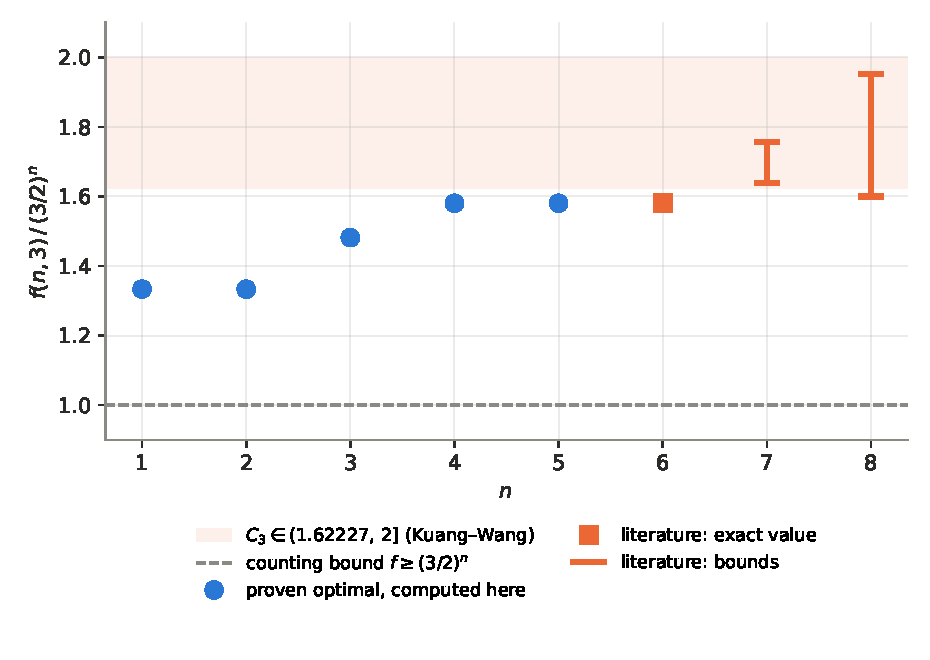
\includegraphics[width=0.8\linewidth]{fig2_covering.pdf}
\caption{Normalized covering numbers $f(n,3)/(3/2)^n$. Circles: proven optimal values computed here ($n\le5$). Square and bars: exact value ($n=6$) and bounds ($n=7,8$) from~\cite{adriaensen2026,kuangwang2026}. The shaded band is the range $1.62227<C_3\le2$ for the limit~\cite{kuangwang2026}; the dashed line is the counting bound.}
\label{fig:covering}
\end{figure}

\begin{corollary}[Rate]
\label{cor:asymp}
For every $n\ge1$,
\[
  \begin{gathered}
  \left\lceil n\log_2(3/2)\right\rceil \;\le\; \Bstar(n,1) \;\le\; \left\lceil n\log_2(3/2)\right\rceil+1,\\
  \text{hence}\qquad \lim_{n\to\infty}\frac{\Bstar(n,1)}{n}=\log_2(3/2)\approx0.585.
  \end{gathered}
\]
\end{corollary}

\begin{proof}
Take $\log_2$ in~\eqref{eq:sandwich}, apply \Cref{thm:main}, and use $\lceil x+1\rceil=\lceil x\rceil+1$. The lower bound uses only the counting bound; the upper bound uses~\cite{kuangwang2026}.
\end{proof}

\begin{corollary}[Non-additivity]
\label{cor:compress}
$\Bstar(1,1)=1$, and $\Bstar(n,1)<n=n\,\Bstar(1,1)$ for every $n\ge4$.
\end{corollary}

\begin{proof}
$\Bstar(1,1)=\lceil\log_2 2\rceil=1$, and $\Bstar(4,1)=3$ by \Cref{tab:finite}. For $n\ge5$, \eqref{eq:sandwich} gives $f(n,3)\le2(3/2)^n<2^{n-1}$, since $4(3/4)^n\le4(3/4)^5=243/256<1$. Hence $\Bstar(n,1)\le n-1$.
\end{proof}

\Cref{fig:frontier} summarizes the exact values. The saving comes from encoding the copies jointly through a cover; it is a classical property of the parallel task, not a quantum effect.

\begin{figure}[H]
\centering
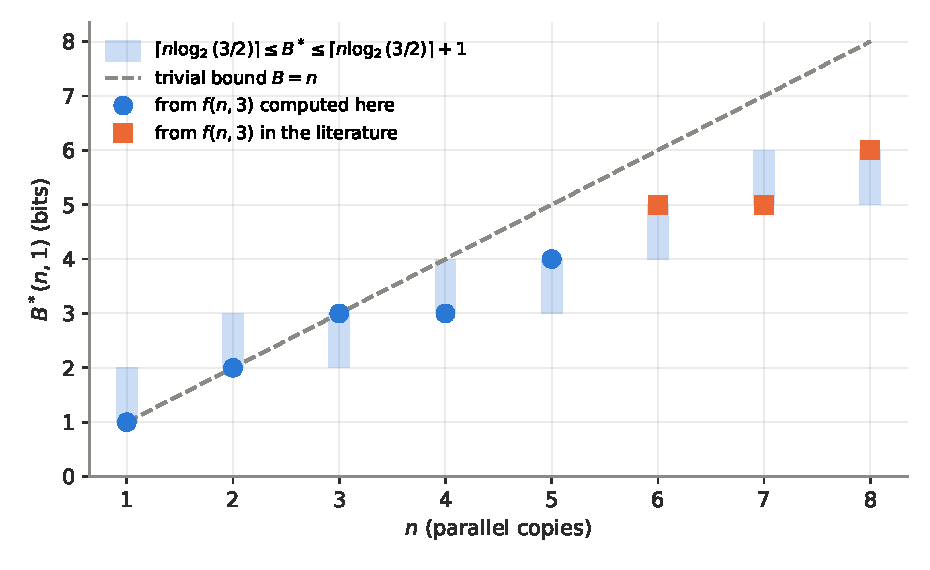
\includegraphics[width=0.8\linewidth]{fig1_frontier.pdf}
\caption{Exact zero-error one-way communication cost $\Bstar(n,1)=\lceil\log_2 f(n,3)\rceil$. Circles use covering numbers computed here, squares use covering numbers from~\cite{adriaensen2026,kuangwang2026}. Shaded bars: the window of \Cref{cor:asymp}. Dashed line: the trivial bound $B=n$ obtained by solving the copies separately.}
\label{fig:frontier}
\end{figure}

\section{Quantum--classical resource comparison}
\label{sec:quantum}

\begin{table}[H]
\centering
\caption{Resources for perfect success. Bits and Bell pairs are different resources; no exchange rate is implied.}
\label{tab:resource}
\begin{tabular}{p{0.23\linewidth}p{0.43\linewidth}p{0.23\linewidth}}
\toprule
 & Classical (deterministic or shared randomness) & Quantum~\cite{zhaodeng2025} \\
\midrule
One-way classical communication & $\Bstar(n,1)=n\log_2(3/2)+O(1)$ bits & $0$ \\
Preshared entanglement & none & $2n$ Bell pairs \\
Success probability & $1$ & $1$ \\
\bottomrule
\end{tabular}
\end{table}

This is a communication--entanglement resource separation: perfect classical success needs $\Theta(n)$ bits of one-way communication, while the quantum protocol needs none. We claim neither a computational speedup nor that a Bell pair replaces a fixed number of bits.

\begin{corollary}[Shared randomness does not help]
\label{cor:shared}
A shared-randomness one-way protocol with $B$ bits and success probability $1$ exists only if a deterministic one exists. Hence $\Bstar_{\mathrm{shared}}(n,1)=\Bstar(n,1)$.
\end{corollary}

\begin{proof}
If $\Pr_{X_A,X_B,R}[W_n=0]=0$, then $\Pr_{X_A,X_B}[W_n=0\mid R=r]=0$ for almost every $r$. Fixing such an $r$ gives a deterministic $B$-bit protocol whose failure probability under the full-support input distribution is $0$, so it wins on every input pair. The converse is trivial.
\end{proof}

\paragraph{Relation to Zhao--Deng.} Zhao and Deng~\cite{zhaodeng2025} prove a constant-versus-linear separation for commonly used classical learning models, using communication lower bounds. We determine a narrower quantity exactly: the zero-error one-way communication. This neither strengthens nor replaces their learning-theoretic theorem.

\section{Related work}
\label{sec:related}

\paragraph{Nonlocality and communication.} Buhrman et al.~\cite{buhrman2010} review the links between nonlocality and communication complexity. Toner and Bacon~\cite{toner2003} showed that one bit of communication suffices to simulate projective measurements on a maximally entangled two-qubit state. The extension to projective measurements on arbitrary two-qubit states was described as open by M\'arton et al.~\cite{marton2024}. Bacon and Toner~\cite{bacon2003} studied Bell inequalities with auxiliary communication. Pseudo-telepathy was formalized by Brassard, Broadbent and Tapp~\cite{brassard2005}, and Cleve et al.~\cite{cleve2004} studied the limits of nonlocal strategies. M\'arton et al.~\cite{marton2024} computed one-bit classical bounds for parallel repetitions of pseudo-telepathy games and showed that two copies of the magic-square game violate the bidirectional one-bit classical bound. We instead determine the exact zero-error one-way cost for all $n$ in the Zhao--Deng task.

\paragraph{Domination and ternary coverings.} Rall~\cite{rall2005} initiated the study of total domination in direct products and proved $\gammat(G\times H)\le\gammat(G)\gammat(H)$ for graphs without isolated vertices. Meki\v{s}~\cite{mekis2010} gave lower bounds for the domination and total domination numbers of direct products of graphs. Adriaensen et al.~\cite{adriaensen2026} introduced the skirting problem (a smallest $S\subseteq\Z_q^n$ such that every point is at Hamming distance $n$ from some element of $S$), identified it with total domination in $K_q^{\times n}$, and computed $f(n,3)$ for $n\le6$ together with $28\le f(7,3)\le30$. Kuang and Wang~\cite{kuangwang2026} proved the asymptotics used in \Cref{sec:finite} and the bounds $41\le f(8,3)\le50$.

\section{Discussion}
\label{sec:discussion}

The zero-error one-way communication complexity of the Zhao--Deng task is governed by a purely combinatorial invariant, and is known to within one bit for every $n$. Parallel copies can be encoded jointly at an asymptotic cost of $\log_2(3/2)\approx0.585$ bits per copy instead of one. The optimal protocol has a particularly simple form (\Cref{rem:structure}).

The no-communication value is \emph{not} multiplicative: $S_1(0)=15/16$, but $S_2(0)\ge227/256>(15/16)^2$ (\Cref{app:nocomm}). This is consistent with known non-multiplicativity for parallel magic-square games~\cite{marton2024}. It does not affect the zero-error results, which concern success probability exactly $1$.

\paragraph{Scope.} The results cover deterministic and shared-randomness one-way protocols with perfect success. Imperfect success ($q<1$), interactive communication and other pseudo-telepathy-derived tasks are left open.

\section{Methods}
\label{sec:methods}

The computational pipeline was rerun for this submission using Python~3.12.15, NumPy~2.3.5 and SciPy~1.18.0 with the bundled HiGHS mixed-integer linear programming (MILP) solver. Figure generation used Matplotlib~3.10.8. Runtime versions, code hashes, full logs and raw solver outputs are archived. MILP runs use one solver thread, a fixed random seed and a requested relative gap of zero. ``Proven optimal'' refers to HiGHS' optimal status at its floating-point tolerances; this is not an independently checked exact-arithmetic certificate. Returned covers and strategy pairs are checked combinatorially.

\paragraph{Single copy} (\texttt{single\_copy.py}). Enumerates all $4^4\times4^4=65\,536$ deterministic strategy pairs and all strategies for the sets in \Cref{lem:single}. It confirms $S_1(0)=15/16$, the $64$ winning strategy pairs for each two-element set, none for $\Hd$, and that every row of \Cref{tab:strategies} wins on all inputs.

\paragraph{Covering numbers} (\texttt{covering\_ilp.py}). One binary variable $z_c$ per $c\in\Z_3^n$, constraints $\sum_{c:\,x\in Q_c}z_c\ge1$ for all $x\in\Z_3^n$, objective $\min\sum_c z_c$. This set-cover formulation is identical to the total-domination formulation. Each returned cover is checked independently. For $n=1,\dots,5$ the solver proved optimality ($f=2,3,5,8,12$). For $n=6$, with a 120\,s limit, it did not (the archived run returned a cover of size $\CoverSixIncumbent$ and a lower bound of $\CoverSixLower$). We therefore take $f(6,3)=18$ from~\cite{adriaensen2026}. Time-limited incumbents and bounds may vary between environments.

\paragraph{Protocol check} (\texttt{protocol\_check.py}). For $n=1,\dots,5$, the protocol of \Cref{thm:main} built from the optimal covers was run on all $4^n\cdot4^n$ input pairs (up to $1\,048\,576$ pairs for $n=5$) and won on all of them, using $\lceil\log_2 f(n,3)\rceil$ bits. This checks the upper bound; the matching lower bound is the proof of \Cref{thm:main}.

\paragraph{No communication, $n=2$} (\texttt{no\_comm\_n2.py}). Alternating best-response search over deterministic strategy pairs (4000 random restarts, seed $0$). The best pair found wins on $\NtwoHeuristic$ of $256$ input pairs; it is listed in the repository and re-scored by an independent routine. \texttt{no\_comm\_n2\_exact.py} formulates the exact discrete problem as a MILP. The archived $1200$\,s run returned incumbent $\NtwoIncumbent$ and the conservative integer upper bound $\NtwoUpper$ (status ``\NtwoStatus''). The raw floating-point objective and dual bound are retained, and no optimality is inferred from an incumbent.

\paragraph{Figures} (\texttt{make\_figures.py}) are generated from the JSON outputs and from a separate file listing the literature values for $n\ge6$.

\subsection*{Use of generative AI}
Generative AI tools (Claude, Anthropic; Devin, Cognition) assisted with language editing, code drafting and review, mathematical checking, and source comparison. During preparation of this submission, the numerical pipeline was executed again and its outputs were checked against the manuscript. The task definition and entanglement count were compared with Zhao--Deng, and the covering theorem was checked against Kuang--Wang's primary text. These AI-assisted checks do not constitute independent human peer review. The author is responsible for the final manuscript and its submission.

\section*{Data and code availability}
All code, raw outputs (including solver status messages) and figure scripts are available at \href{\repoURL}{\nolinkurl{github.com/VesterlundCoder/cqa07-paper-v1.0}} and archived at Zenodo, \href{https://doi.org/\zenodoDOI}{doi:\zenodoDOI}.

\section*{Author contributions}
D.V.: conceptualization, mathematical derivation, software, verification, visualization, writing.

\section*{Funding}
This research received no external funding.

\section*{Ethics approval and consent}
Not applicable. This theoretical and computational study involved no human participants, animals or personal research data.

\section*{Competing interests}
The author declares no competing interests.

\appendix

\section{No-communication baseline}
\label{app:nocomm}

\paragraph{One copy.} Exhaustive enumeration gives $S_1(0)=15/16$. One loss among the $16$ input pairs is unavoidable by \Cref{lem:single}.

\paragraph{Two copies.} Using the optimal single-copy strategy in each copy gives $S_2(0)\ge(15/16)^2=225/256$. A correlated deterministic strategy pair found by search wins on $227$ input pairs, so
\[
  S_2(0)\;\ge\;227/256\;>\;(15/16)^2 .
\]
The strategy pair is listed in \texttt{data/no\_comm\_n2.json}. The exact discrete problem was also formulated as a MILP (\texttt{no\_comm\_n2\_exact.py}). The archived run has status ``\NtwoStatus'' and yields the solver upper bound $\NtwoUpper$, so $227/256\le S_2(0)\le\NtwoUpper/256$. A complete deterministic strategy wins on an integer number of input pairs, so the raw dual bound is rounded down, allowing a $10^{-6}$ numerical tolerance, when reporting this integer bound. This numerical upper bound is separate from the explicitly verified lower-bound strategy and from the analytic zero-error theorem.
Consequently $S_n(0)\ge(227/256)^{n/2}$ for even $n$, so $S_n(0)$ is not multiplicative under parallel repetition. Its exact value for $n\ge2$ is not needed for the results above.

\begin{thebibliography}{99}

\bibitem{zhaodeng2025}
Zhao, H. \& Deng, D.-L. Entanglement-induced provable and robust quantum learning advantages. \emph{npj Quantum Inf.} \textbf{11}, 127 (2025). \href{https://doi.org/10.1038/s41534-025-01078-x}{doi:10.1038/s41534-025-01078-x}.

\bibitem{adriaensen2026}
Adriaensen, S., Ihringer, F., Martin, W.~J. \& Villagr\'an, R.~R. Skirting the $n$-tuples. arXiv:2602.01080v1 (2026). \url{https://arxiv.org/abs/2602.01080v1}.

\bibitem{kuangwang2026}
Kuang, P. \& Wang, Y. Covering the ternary cube by binary subcubes. arXiv:2608.13252v1 (2026), Theorem~1.2. \url{https://arxiv.org/abs/2608.13252v1}.

\bibitem{rall2005}
Rall, D.~F. Total domination in categorical products of graphs. \emph{Discuss. Math. Graph Theory} \textbf{25}, 35--44 (2005).

\bibitem{mekis2010}
Meki\v{s}, G. Lower bounds for the domination number and the total domination number of direct product graphs. \emph{Discrete Math.} \textbf{310}, 3310--3317 (2010).

\bibitem{marton2024}
M\'arton, I., Bene, E., Divi\'anszky, P. \& V\'ertesi, T. Beating one bit of communication with and without quantum pseudo-telepathy. \emph{npj Quantum Inf.} \textbf{10}, 79 (2024).

\bibitem{buhrman2010}
Buhrman, H., Cleve, R., Massar, S. \& de Wolf, R. Nonlocality and communication complexity. \emph{Rev. Mod. Phys.} \textbf{82}, 665--698 (2010).

\bibitem{toner2003}
Toner, B.~F. \& Bacon, D. Communication cost of simulating Bell correlations. \emph{Phys. Rev. Lett.} \textbf{91}, 187904 (2003).

\bibitem{bacon2003}
Bacon, D. \& Toner, B.~F. Bell inequalities with auxiliary communication. \emph{Phys. Rev. Lett.} \textbf{90}, 157904 (2003).

\bibitem{cleve2004}
Cleve, R., H{\o}yer, P., Toner, B. \& Watrous, J. Consequences and limits of nonlocal strategies. In \emph{Proc. 19th IEEE Conf. Computational Complexity} 236--249 (2004).

\bibitem{brassard2005}
Brassard, G., Broadbent, A. \& Tapp, A. Quantum pseudo-telepathy. \emph{Found. Phys.} \textbf{35}, 1877--1907 (2005).

\bibitem{mermin1990}
Mermin, N.~D. Simple unified form for the major no-hidden-variables theorems. \emph{Phys. Rev. Lett.} \textbf{65}, 3373--3376 (1990).

\bibitem{peres1990}
Peres, A. Incompatible results of quantum measurements. \emph{Phys. Lett. A} \textbf{151}, 107--108 (1990).

\end{thebibliography}

\end{document}
